\label{sec:studyDesign}
In this sub-section, we describe the details of the data collection and processing approach followed to answer our different research questions.





\subsection{Data Collection}
\label{sec:dataCollection}
Le développement du système de détection d'odeurs de conception s'est fait à
partir des exemples de code de programmes d'apprentissage profond. Ces exemples
représentent des programmes d'apprentissage profond dans lesquels on y trouve
des odeurs de conceptions. Ses exemples ont été collectés par Nikanjam et al.
\cite{nikanjam2021design} dans
le cadre de leur étude empirique sur les odeurs de conception dans les
programmes d'apprentissage profond. En effet, dans cette étude, ils
ont présenté des exemples de programmes d'apprentissage profond contenant les
ordeurs de conceptions énumérées dans l'introduction \ref{sec:codeSmell}. Ces
exemples de code source ont été collectés à partir des plateformes StackOverflow
et Github.\\\\

Le système de détection d'odeurs de conception ainsi développé a servi sur un
ensemble de programmes d'apprentissage profond collectés à partir de la
plateforme Github. Ces programmes d'apprentissage profond ont été collectés
selon un processus bien défini. En effet, nous avons utilisé l'API de Github et
plus précisement les requêtes de recherche de type \emph{search code}. Cette requête
permet de rechercher des fichiers dans les dépôts Github contenant des mots clés
spécifiques définis dans notre système. Étant donné que notre papier se
concentre uniquement sur les libraires \emph{Keras}, \emph{Tensorflow} et \emph{Pytorch}, nous avons utilisé les mots
clés présentés dans le tableau \ref{tab:keywords}. Ces mots clés
représentent les modules et les fonctions de ces trois librairies.\\


\begin{table}[h]
  \centering
  \caption{\emph{Liste des mots clés utilisés pour la recherche de programmes d'apprentissage profond dans les dépôts Github.}}
  \label{tab:keywords}
  \begin{tabular}{ll}
    \toprule
    \textbf{Mots clés}         & \textbf{Librairie} \\ \midrule
    keras.layers               & Keras              \\
    keras.layers.convolutional & Keras              \\
    AveragePooling2D           & Keras/Tensorflow   \\
    MaxPooling2D               & Keras/Tensorflow   \\
    tensorflow.keras.layers    & Tensorflow         \\
    Conv2D                     & Keras/Tensorflow   \\
    Convolution2D              & Keras/Tensorflow   \\
    BatchNormalization         & Keras/Tensorflow   \\
    import torch               & Pytorch            \\
    import torchvision.models  & Pytorch            \\
    torch.nn.Sequential        & Pytorch            \\
    torch.nn.Conv2d            & Pytorch            \\
    torch.nn.BatchNorm2d       & Pytorch            \\
    torch.nn.MaxPool2d         & Pytorch            \\ \bottomrule
  \end{tabular}
\end{table}


La requête de recherche de type \emph{search code} retourne un ensemble
d'informations sur le repository et le fichier contenant les mots clés
recherchés. Cette collecte retourne un ensemble de données brute de 9572
repositories Github diférents. Nous sélectionnons ensuite aléatoirement un sous
ensemble de 10\% de notre ensemble de données brutes, soit 958 repositories
Github afin d'optimiser l'étape de filtrage manuel ci-après.

À partir de ce sous ensemble, nous procédons ensuite à un filtrage des répertoires selon les
critères suivants: (1) nombre de commit ($\geq$ 100), (2) nombre d'étoile ($\geq$ 100), (3) dernière date du
commit($\leq$ 5 years), (4) nombre de contributeurs ($\geq$ 5). Ce filtrage nous permet de ne garder que
les répertoires qui sont les plus populaires et qui sont les plus actifs. Nous
avons ensuite procédé à un filtrage manuel des répertoires en éliminant les
projets qui ne sont pas des programmes d'apprentissage profond ou ne pas
pertinente pour notre étude (n'utilise pas les librairies choisies, ou
n'implémente pas de réseau de neurones). De ce fait nous nous sommes retrouvé
avec 500 projets sur lesquels nous allons appliquer notre système de détection
d'odeurs de conception.\\ Le schema \ref{fig:data_collect} présente le processus
de collecte des programmes d'apprentissage profond.\\

\begin{figure*}[h]
  \centering
  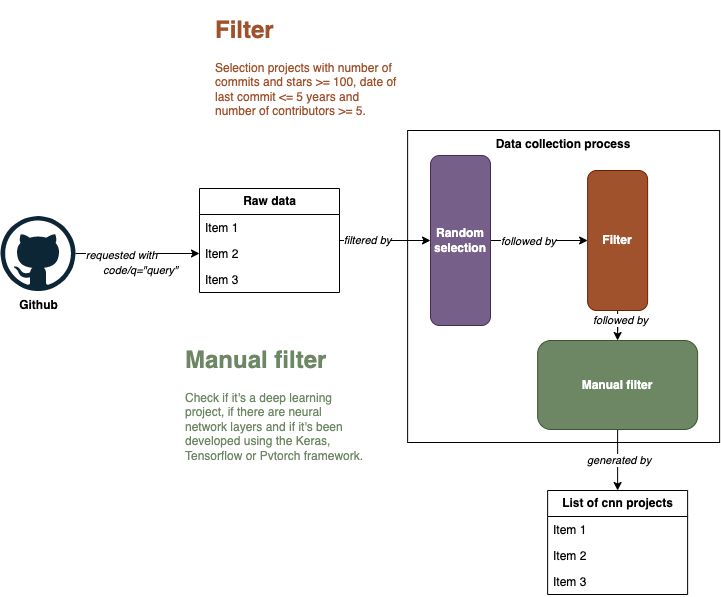
\includegraphics[width=0.8\textwidth]{figure/design_smell_data_collection.png}
  \caption{\emph{Processus de collecte des projets d'apprentissage profond dans Github.}}
  \label{fig:data_collect}
\end{figure*}






\subsection{Data Processing}
\label{sec:DataProcessing}
Le processus de collecte des programmes d'apprentissage profond nous a permis
d'avoir un ensemble de programmes d'apprentissage profond sur lesquels nous
allons appliquer notre système de détection d'odeurs de conception. Cependant,
il est important de noter que les programmes d'apprentissage profond sont dans
notre cas des programmes uniquement écrits en langage Python. Il est donc
essentiel de noter que, le système de détection d'odeurs de conception développé
dans ce papier est un système qui est uniquement capable de détecter les odeurs de
conception dans les programmes d'apprentissage profond écrits en langage
Python.\\

Afin de répondre à la question de recherche \emph{RQ1}, nous avons développé un système de détection d'odeurs de
conception dans les programmes d'apprentissage profond. Ce système se décompose
en trois parties. La première partie est la partie relative à la
modélisation des programmes d'apprentissage profond. La
deuxième partie est celle relative à la détection des odeurs de conception
dans les programmes d'apprentissage profond. Et la troisième est la partie
relative à l'analyse des résultats de la détection.\\

\subsubsection{Modélisation des programmes d'apprentissage profond}
\label{sec:Meta-modélisation des programmes d'apprentissage profond}
La modélisation des programmes d'apprentissage profond est la première
étape du processus de détection des odeurs de conception. Cette étape consiste à transformer le code source des programmes
d'apprentissage profond collecté en un modèle intermédiaire qui sera utilisé pour la
détection des odeurs de conception. Ce modèle intermédiaire est un modèle de
type \emph{Famix Abstract Syntax Tree} (\emph{FAST}) \ref{fig:fast}. Le modèle \emph{FAST} est un modèle qui
est utilisé pour représenter les programmes sous forme d'arbre syntaxique. Il
hérite de la représentation abstraite de codes sources \emph{Famix} dévéloppé
dans le langage de programmation \emph{Pharo}. Avec \emph{Famix}, le code
source est représenté sous forme d'objet et selon un métamodèle défini pour symplifier l'analyse et
la représentation de programmes complexes. Un modèle \emph{Famix} est une
représentation agnostique en terme de langage du code source d'origine et embarque des
fonctions qui permettent entre autres sa navigation et sa transformation.\\

La transformation du code source collecté en modèle \emph{FAST} se fait comme suit.
Chaque projet collecté est cloné dans un répertoire local. Son code source est
ensuite parsé à l'aide de la librairie \emph{ast.py} de Python. Cette librairie
permet de transformer le code source en un arbre syntaxique sous forme \emph{json}. Le
\emph{json} obtenu est ensuite transformé en un modèle \emph{FAST} à l'aide d'un importateur
développé sous le patron de conception visiteur. Les visiteurs sont des fonctions
qui permettent de parcourir un arbre syntaxique pour effectuer sur ses noeuds des opérations
spécifiques. Dans notre cas, nous avons développé des visiteurs qui
nous permettent de parcourir l'arbre syntaxique (\emph{json}) et de transformer chaque
noeud de cet arbre en une entité de \emph{FAST}.\\

Le schema \ref{fig:modelling} illustre le processus de modélisation des
programmes d'apprentissage profond.\\

\begin{figure*}[h]
  \centering
  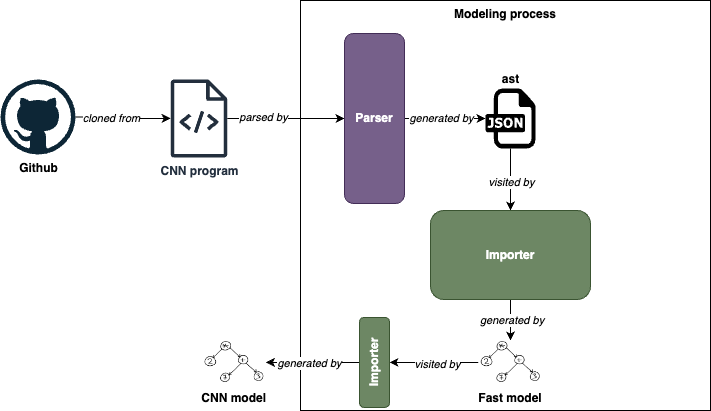
\includegraphics[width=0.8\textwidth]{figure/design_smell_modeling.png}
  \caption{\emph{Processus de modeling des projets d'apprentissage profond.}}
  \label{fig:modelling}
\end{figure*}


\subsubsection{Détection des odeurs de conception}
\label{sec:Detection des odeurs de conception}
Le modèle \emph{FAST} obtenu à partir de la modélisation des programmes
d'apprentissage profond est ensuite utilisé pour la détection des odeurs de
conception. Cette étape consiste à parcourir le modèle \emph{FAST} et à appliquer les
règles de détection des odeurs de conception. Ces règles sont définies
dans le langage de programmation \emph{Pharo}.\\ Une règle ou plusieurs règles
peuvent être appliquées sur un noeud de l'arbre syntaxique afin de détecter une
odeur de conception.\\

% Le schema \ref{fig:rules} est un exemple de règle
% permettant de détecter l'odeur de conception numéro 5 - \emph{Non-dominating down-sampling}.\\
Le schema \ref{fig:detection} illustre le processus de détection des odeurs de conception.\\


\begin{figure*}[h]
  \centering
  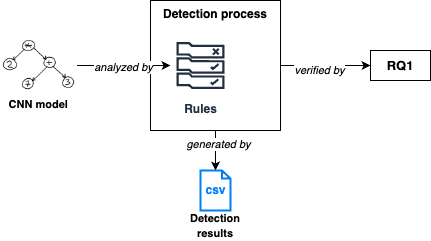
\includegraphics[width=0.8\textwidth]{figure/design_smell_detection.png}
  \caption{\emph{Processus de détection des odeurs de conception.}}
  \label{fig:detection}
\end{figure*}

\subsubsection{Analyse des résultats de la détection des odeurs de conception}
\label{sec:Analyse des résultats de la détection des odeurs de conception}
Les résultats de la détection des odeurs de conception de chaque repository sont
stockés sous forme \emph{csv}. Pour chaque repository nous enregistrons le nom de
chaque odeur de conception détectée, le nombre de fois que cette odeur est
détectée dans un fichier du repository et le chemin de ce fichier. Ces résultats
permettent de répondre aux questions de recherche \emph{RQ2} et \emph{RQ3}.\\
On calcul ensuite la répartition des odeurs de conception dans chaque repository
en divisant le nombre de fois qu'une odeur de conception est détectée par le
nombre total d'odeurs de conception détectées dans le repository. Cette
répartition permet de répondre à la question de recherche \emph{RQ2}. On
calcul également la répartition des odeurs de conception dans l'ensemble des 500
repositories en divisant le nombre de fois qu'une odeur de conception est
détectée par le nombre total d'odeurs de conception détectées dans l'ensemble
des 500 repositories. Cette répartition permet aussi de répondre à la
question de recherche \emph{RQ2}.\\

On calcul ensuite la matrice de corrélation entre les odeurs de conception dans
l'ensemble des 500 repositories. Cette matrice permet de répondre à la question
de recherche \emph{RQ3}. Une matrice de corrélation permet
de calculer la corrélation entre deux variables.

Un coeficient de corrélation est calculé à l'aide de la formule suivante:  $r =
  \frac{cov(X,Y)}{\sigma_X \sigma_Y}$  où $r$ est le coeficient de corrélation, $cov(X,Y)$ est la covariance entre les
deux variables $X$ et $Y$, $\sigma_X$ est l'écart type de la variable $X$ et
$\sigma_Y$ est l'écart type de la variable $Y$. Ce coeficient de corrélation est
compris entre -1 et 1. On parle de correlation positive lorsque le coeficient de
corrélation est compris entre 0 et 1. Dans ce cas, plus il est proche de 1, plus les deux variables sont
corrélées positivement, et plus il est proche de 0, moins les deux variables sont
corrélées. On parle de correlation négatif lorsque le coeficient de corrélation
est compris entre -1 et 0. Dans ce cas, plus le coeficient de corrélation est
proche de -1, plus les deux variables sont corrélées négativement, et plus il
est proche de 0, moins les deux variables sont corrélées.\\



Dans notre cas, les variables sont les odeurs de conception. La corrélation entre deux odeurs de conception est
calculée en divisant le nombre de fois que les deux odeurs de conception sont
détectées ensemble par le nombre total de fois que les deux odeurs de conception
sont détectées. Cette corrélation est calculée pour chaque paire d'odeurs de
conception. Plus elle est proche de 1, plus les deux odeurs de conception sont
corrélées, et plus elle est proche de 0, moins les deux odeurs de conception
sont corrélées.\\

Une corrélation positive signifie que les deux odeurs de conception
sont souvent détectées ensemble. Et une corrélation négative signifie que les deux odeurs de conception sont rarement
détectées ensemble. Enfin une corrélation nulle signifie que les deux odeurs de
conception ne sont jamais détectées ensemble.\\

Le schema \ref{fig:analysis} illustre le processus de cette dernière partie.\\

\begin{figure*}[h]
  \centering
  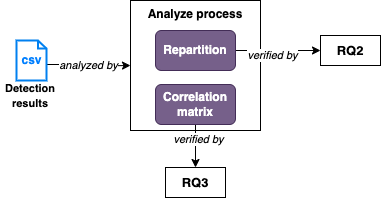
\includegraphics[width=0.8\textwidth]{figure/design_smell_analyze.png}
  \caption{\emph{Processus d'analyse des résultats de la détection des odeurs de conception.}}
  \label{fig:analysis}
\end{figure*}

\subsection{Replication Package}
\label{sec:Replication Package}
Le code source du parse de code source en arbre de Syntax \emph{json} est sur
Github à l'adresse \url{https://github.com/aurpur/parserPythonToJson} et celui du
système de détection d'odeurs est disponible sur Github à l'adresse
\url{https://github.com/aurpur/famixPythonImporter}. Le système
de collection de données est aussi disponible sur Github à l'adresse
\url{https://github.com/aurpur/ms-github-data-collection}.\\
